\documentclass{article}
\usepackage[utf8]{inputenc}
\usepackage{amsmath}
\usepackage{graphicx}
\usepackage{subcaption}
\usepackage{float}
\usepackage{geometry}
\geometry{a4paper, margin=1in}

\title{SH1017 Physics for Engineering Mathematics \\ Computer Lab 2: Diffraction and Interference}
\author{--}
\date{\today}

\begin{document}

\maketitle

\section*{Background}
This report details the findings from Computer Lab 2, focusing on the simulation of wave interference and diffraction using point sources. We investigate the behavior of interference patterns as we vary source configurations, slit widths, and distances. The electric field $E(\mathbf{r}, t)$ from $N$ identical sources at positions $\mathbf{r}_i$ is given by the superposition:
\begin{equation}
E(\mathbf{r}, t) = \sum_{i=1}^{N} \frac{A}{|\mathbf{r} - \mathbf{r}_i|} \cos(k|\mathbf{r} - \mathbf{r}_i| - \omega t)
\end{equation}
The time-averaged intensity measured on a detector screen at distance $D$ is:
\begin{equation}
\overline{E^2} = \frac{|A|^2}{r^2} \left( \frac{N}{2} + \sum_{i=1}^{N-1} \sum_{j=i+1}^N \cos(k|\mathbf{r} - \mathbf{r}_i| - k|\mathbf{r} - \mathbf{r}_j|) \right)
\end{equation}

\section*{Q1: Interference from Point Sources}

\textbf{Method:} Using \texttt{interference.py}, we simulate two coherent point sources and observe how the interference pattern changes with the separation distance $d$ and by adding a third source.

\begin{figure}[H]
    \centering
    \begin{subfigure}[b]{0.45\textwidth}
        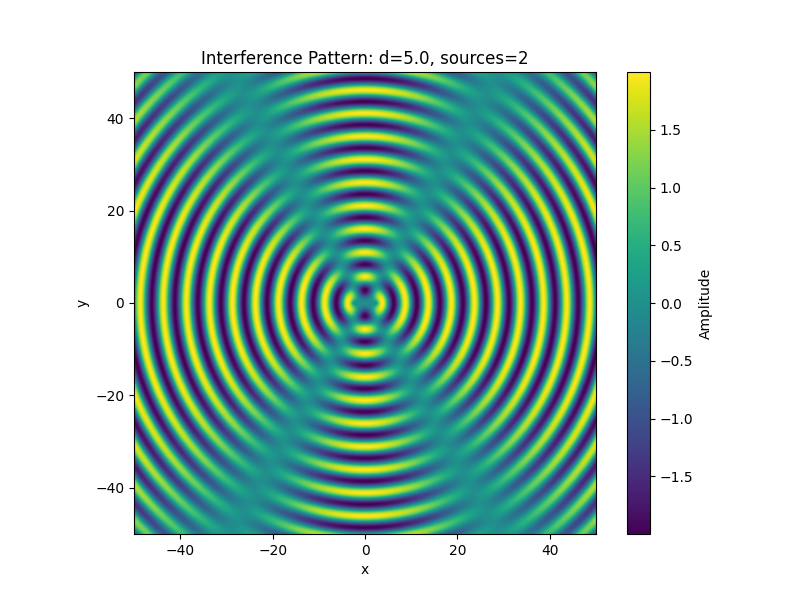
\includegraphics[width=\textwidth]{figures/p1_d10.png}
        \caption{$d=5$}
    \end{subfigure}
    \begin{subfigure}[b]{0.45\textwidth}
        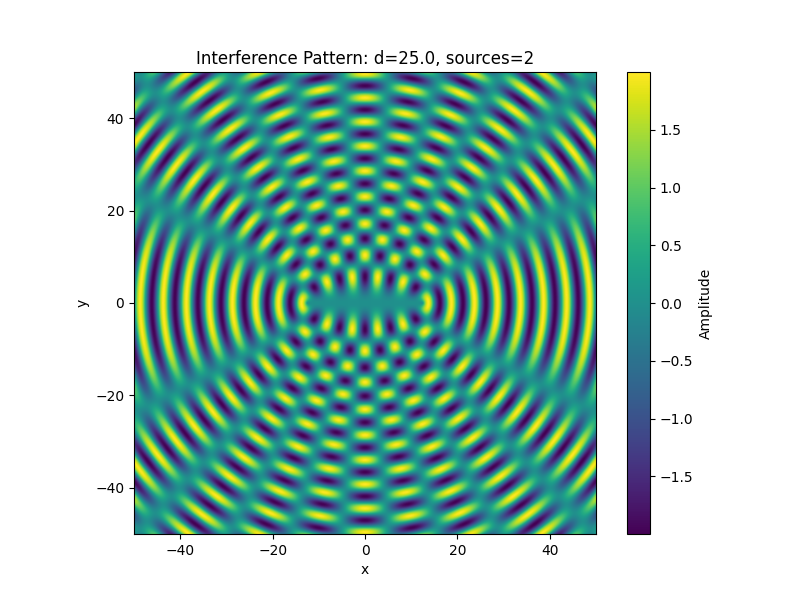
\includegraphics[width=\textwidth]{figures/p1_d20.png}
        \caption{$d=25$}
    \end{subfigure}
    \begin{subfigure}[b]{0.45\textwidth}
        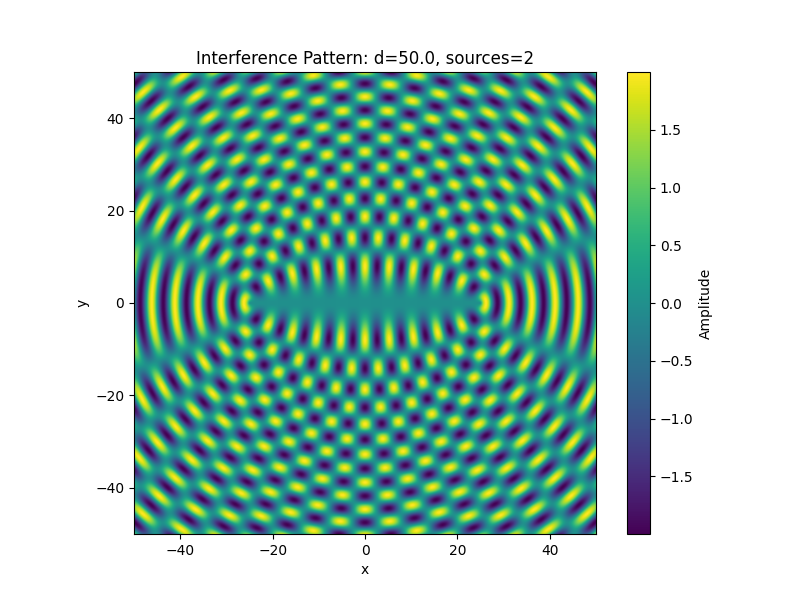
\includegraphics[width=\textwidth]{figures/p1_d40.png}
        \caption{$d=50$}
    \end{subfigure}
    \begin{subfigure}[b]{0.45\textwidth}
        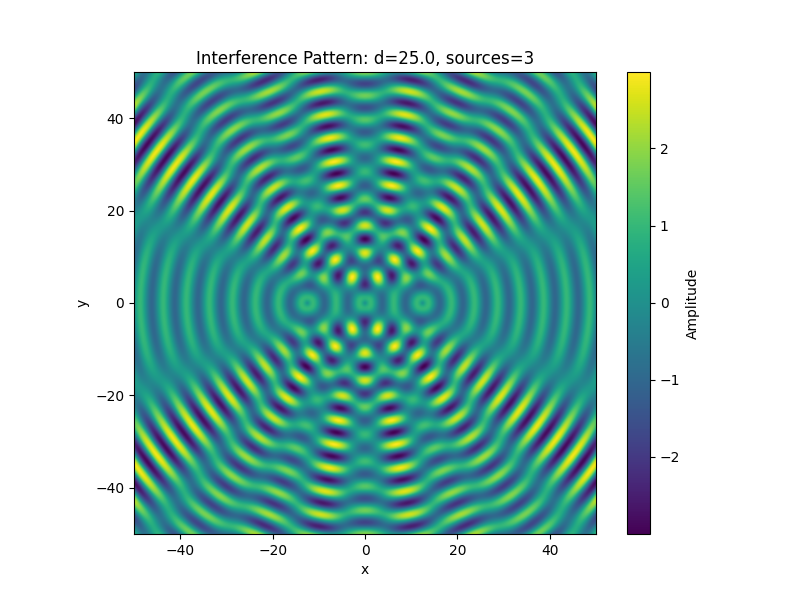
\includegraphics[width=\textwidth]{figures/p1_3sources.png}
        \caption{3 sources, $d=25$}
    \end{subfigure}
    \caption{Interference patterns for different configurations ($\lambda=5.0$ mm, $100 \times 100$ mm area).}
    \label{fig:p1}
\end{figure}

% \textbf{Theory:} According to $N$-slit interference theory, increasing the distance $d$ between sources should decrease the angular separation between fringes, leading to more fringes within a given area. Adding more sources 
% should sharpen the primary maxima and introduce more smaller maxima between them.

\textbf{Results:} As seen in Figure \ref{fig:p1}, increasing the distance $d$ between the 
sources increases the number of interference fringes (maxima and minima) within the same area, corresponding to a smaller angular separation. Adding a third source between the two existing ones sharpens the primary maxima and introduces secondary, smaller maxima between them. These observations are consistent with theoretical predictions.

\section*{Q2: Double Slit Interference}

\textbf{Method:} Using the code from \texttt{doubleslit.py}, we simulate the interference pattern on a screen at distance $D$ from two slits separated by $d$, using $\lambda = 500$ nm. 

\begin{figure}[H]
    \centering
    \begin{subfigure}[b]{0.8\textwidth}
        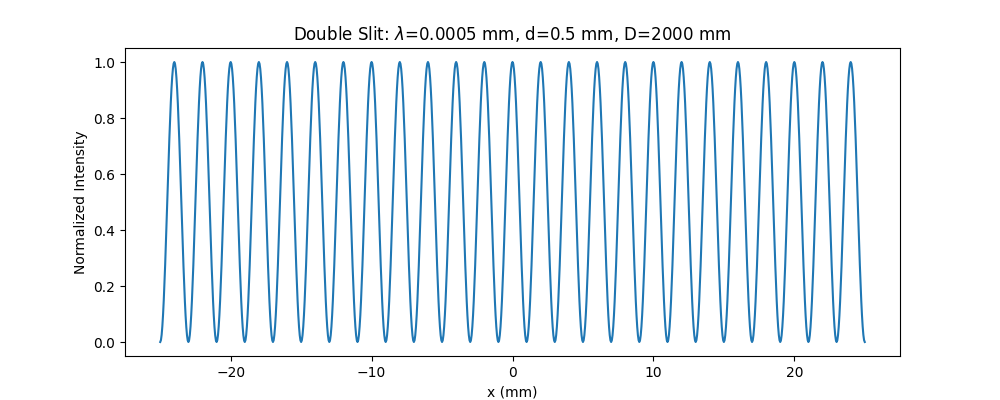
\includegraphics[width=\textwidth]{figures/p2_base.png}
        \caption{Base: $\lambda=0.0005$ mm, $d=0.5$ mm, $D=2000$ mm}
    \end{subfigure}
    \begin{subfigure}[b]{0.8\textwidth}
        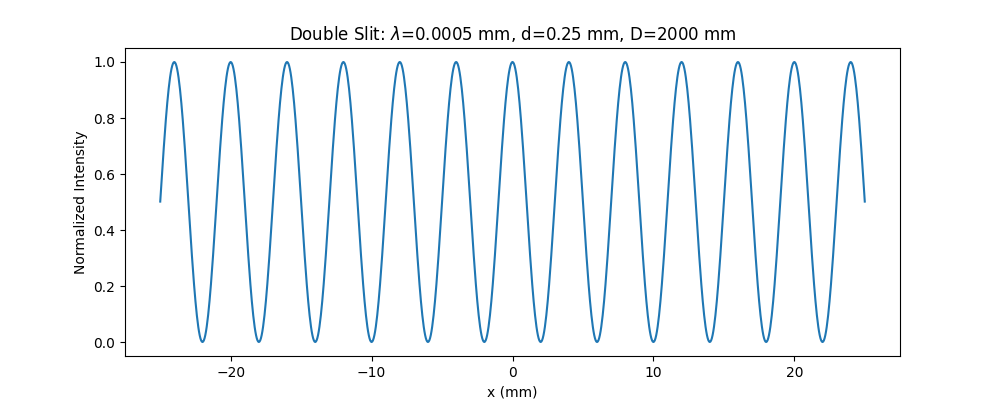
\includegraphics[width=\textwidth]{figures/p2_d_small.png}
        \caption{Smaller $d$: $\lambda=0.0005$ mm, $d=0.25$ mm, $D=2000$ mm}
    \end{subfigure}
    \begin{subfigure}[b]{0.8\textwidth}
        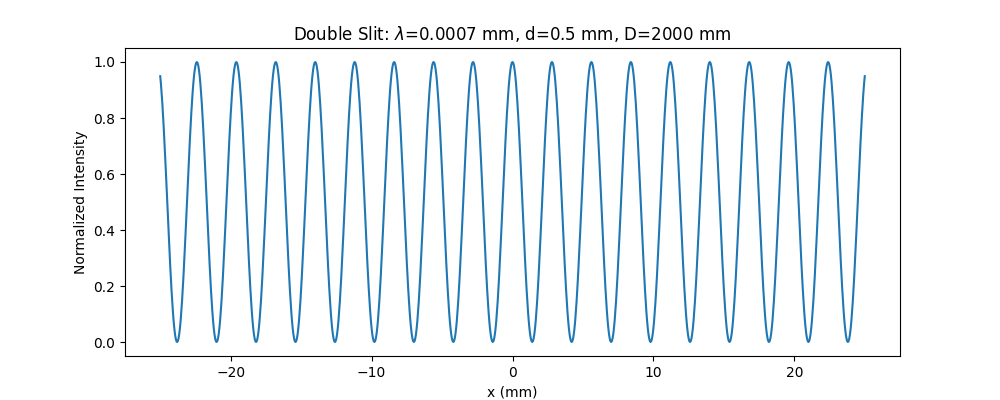
\includegraphics[width=\textwidth]{figures/p2_lambda_red.png}
        \caption{Larger $\lambda$: $\lambda=0.0007$ mm, $d=0.5$ mm, $D=2000$ mm}
    \end{subfigure}

\end{figure}

\textbf{Theory:} The distance between maxima is given by $\Delta x = \lambda D / d$.
and interference order on a flat screen. 
% Without these approximations, the exact geometric distance $r = \sqrt{D^2 + x^2}$ must be considered, 
% meaning the distance between fringes on a flat screen should 
% increase as we move further from the center compared to what 
% the simple formula predicts.

\textbf{Results:} The results for various parameters are summarized below:
\begin{table}[h]
\centering
\begin{tabular}{|l|c|c|c|c|c|}
\hline
Case & $\lambda$ (mm) & $d$ (mm) & $D$ (mm) & Theoretical $\Delta x$ (mm) & Measured $\Delta x$ (mm) \\ \hline
Base & 0.0005 & 0.5 & 2000 & 2.0000 & 2.0000 \\
Larger $\lambda$ & 0.0007 & 0.5 & 2000 & 2.8000 & 2.8000 \\
Smaller $d$ & 0.0005 & 0.25 & 2000 & 4.0000 & 4.0000 \\
Smaller $D$ & 0.0005 & 0.5 & 1000 & 1.0000 & 1.0000 \\
\hline
\end{tabular}

\caption{Comparison of theoretical and measured fringe spacing.}
\label{tab:p2}
\end{table}

The numerical approximation of $\Delta x$ is accurate to the theoretical value within 4 sig figs. And as expected
the frequency increases linearly with both distance to the screen $D$ and wavelength and it decreases with distance between the slits $d$ 

% The measured values differ and are consistently larger than the 
% simple formula $\Delta x = \lambda D / d$. This is because the 
% formula assumes a small-angle approximation ($\sin \theta \approx \theta$) 
% and a planar detector screen, whereas the simulation uses the exact geometric 
% distance $r = \sqrt{D^2 + x^2}$. As $x$ increases, the distance between fringes 
% on a flat screen increases compared to an arc. This geometric effect accounts 
% for the observed deviations from the theoretical approximation.

\section*{Q3: Single Slit Model}

\textbf{Method:} We modify \texttt{doubleslit.py} to approximate a single slit of width $w = 0.05$ mm by placing $N \in \{2, 3, 5, 10\}$ point sources along the slit, using $\lambda = 0.0005$ mm and $D=2000$ mm. We investigate how the peak intensity and width depend on $N$ and $w$.

\begin{figure}[H]
    \centering
    \begin{subfigure}[b]{0.45\textwidth}
        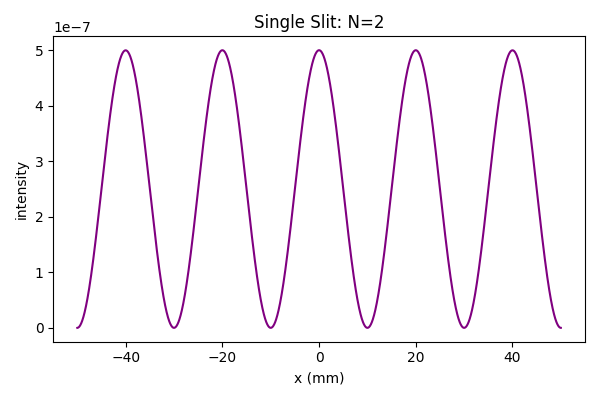
\includegraphics[width=\textwidth]{figures/p3_N2.png}
        \caption{$N=2$}
    \end{subfigure}
    \begin{subfigure}[b]{0.45\textwidth}
        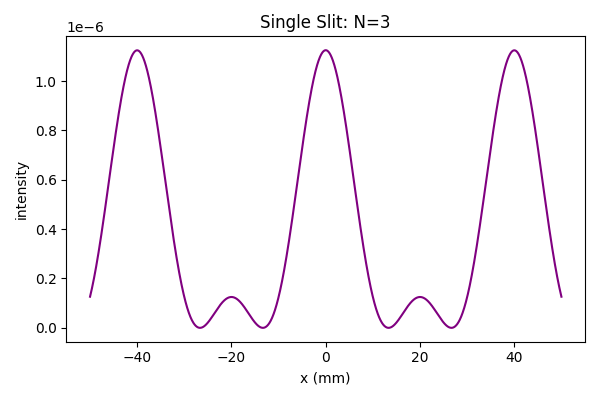
\includegraphics[width=\textwidth]{figures/p3_N3.png}
        \caption{$N=3$}
    \end{subfigure}
    \begin{subfigure}[b]{0.45\textwidth}
        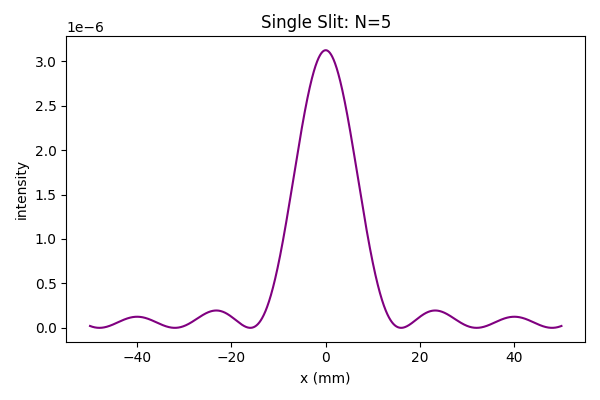
\includegraphics[width=\textwidth]{figures/p3_N5.png}
        \caption{$N=5$}
    \end{subfigure}
    \begin{subfigure}[b]{0.45\textwidth}
        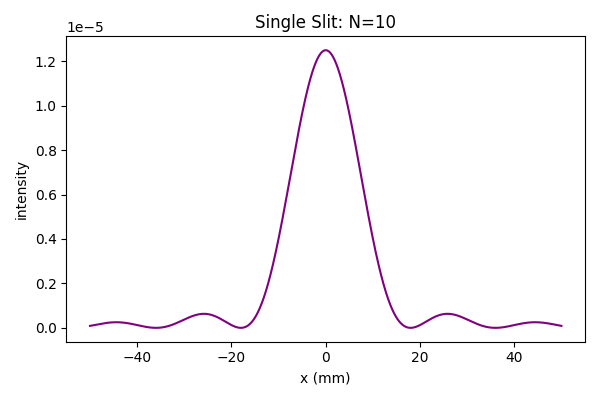
\includegraphics[width=\textwidth]{figures/p3_N10.png}
        \caption{$N=10$}
    \end{subfigure}
    \caption{Intensity distribution for a single slit modeled with varying $N$ sources ($w=0.05$ mm, $\lambda=0.0005$ mm, $D=2000$ mm).}
    \label{fig:p3_N}
\end{figure}

\begin{figure}[H]
    \centering
    \begin{subfigure}[b]{0.45\textwidth}
        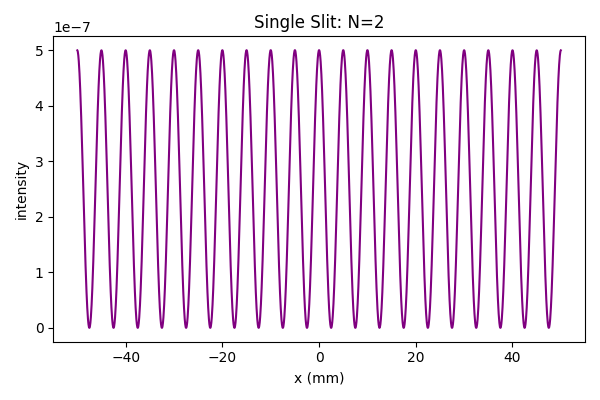
\includegraphics[width=\textwidth]{figures/p3_N_diff_w2.png}
        \caption{$N=2$}
    \end{subfigure}
    \begin{subfigure}[b]{0.45\textwidth}
        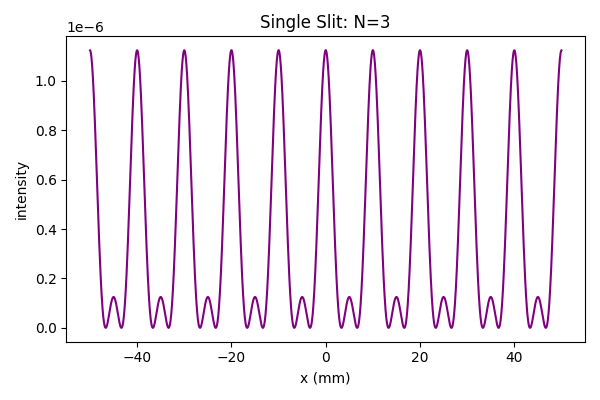
\includegraphics[width=\textwidth]{figures/p3_N_diff_w3.png}
        \caption{$N=3$}
    \end{subfigure}
    \begin{subfigure}[b]{0.45\textwidth}
        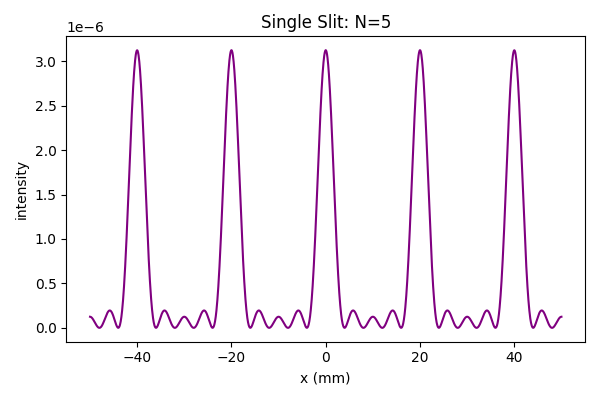
\includegraphics[width=\textwidth]{figures/p3_N_diff_w5.png}
        \caption{$N=5$}
    \end{subfigure}
    \begin{subfigure}[b]{0.45\textwidth}
        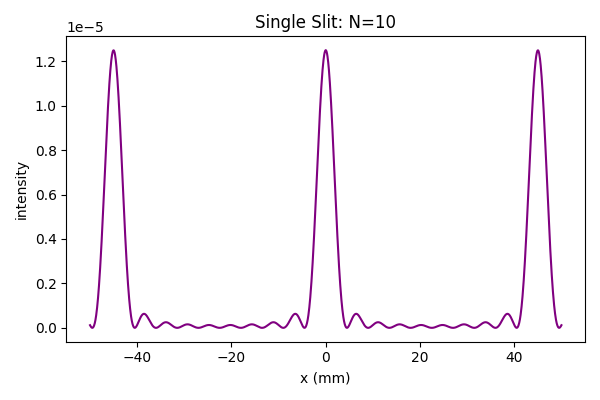
\includegraphics[width=\textwidth]{figures/p3_N_diff_w10.png}
        \caption{$N=10$}
    \end{subfigure}
    \caption{Intensity distribution for a single slit modeled with varying $N$ sources ($w=0.2$ mm, $\lambda=0.0005$ mm, $D=2000$ mm).}
    \label{fig:p3_w}
\end{figure}

\textbf{Theory:} Adjusting the number of point sources $N$ inside a fixed slit width $w$ determines how well we approximate a continuous slit. As $N$ increases, the peak intensity at the center ($x=0$) should scale quadratically (proportional to $N^2$) because the $N$ coherent waves perfectly constructively interfere. The pattern should also converge to display distinct side lobes characteristic of a continuous single slit. Furthermore, diffraction theory predicts that the angular width of the central diffraction peak is inversely proportional to the slit width $w$ (specifically, the angular spread $\theta \approx \lambda/w$). Thus, widening the slit $w$ will result in a narrower central peak, while narrowing $w$ will yield a wider central peak.

\textbf{Results:} As seen in Figure \ref{fig:p3_N} ($w=0.05$ mm), increasing $N$ causes the central peak intensity to grow quadratically, which is consistent with the expected $N^2$ scaling behavior (for example, the peak for $N=10$ is approximately 25 times taller than the peak for $N=2$). Moreover, as $N$ increases to 10, the pattern evolves to exhibit secondary side lobes, approaching a continuous single-slit diffraction envelope. 

Figure \ref{fig:p3_w} demonstrates the same variation in $N$ but for a wider slit ($w=0.2$ mm). Comparing the fully developed patterns ($N=10$) between Figure \ref{fig:p3_w} and Figure \ref{fig:p3_N}, the central peak for $w=0.2$ mm is narrower than for $w=0.05$ mm, and its side lobes are packed more tightly together. These observations provide evidence that the peak width is inversely proportional to the slit width $w$, which is consistent with the scaling and interference principles of single-slit diffraction theory.

\section*{Q4: Realistic Double Slit Model}

\textbf{Method:} We copied 2 of the "realistic" slits from problem 3 ($N=10$, $w=0.05$ mm) and separated them by $d=0.5$ mm and compared it to the point-source model.

\begin{figure}[H]
    \centering
        \begin{subfigure}[b]{0.8\textwidth}
        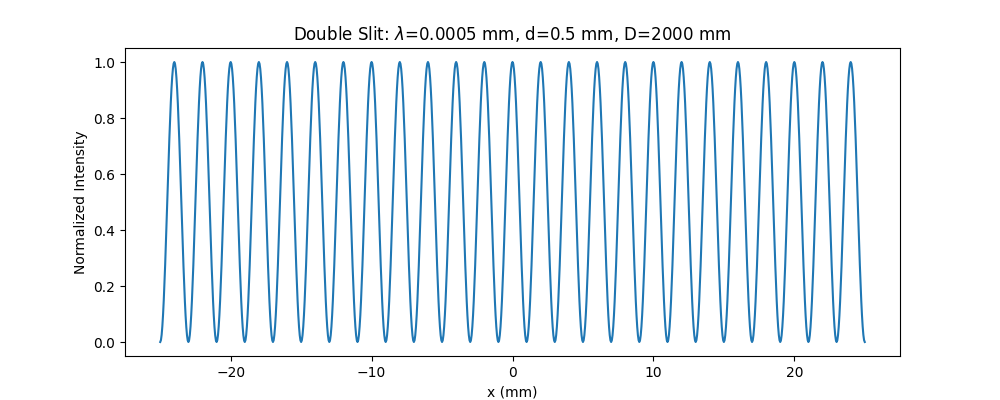
\includegraphics[width=\textwidth]{figures/p2_base.png}
        \caption{Point source model}
    \end{subfigure}
    \begin{subfigure}[b]{0.8\textwidth}
        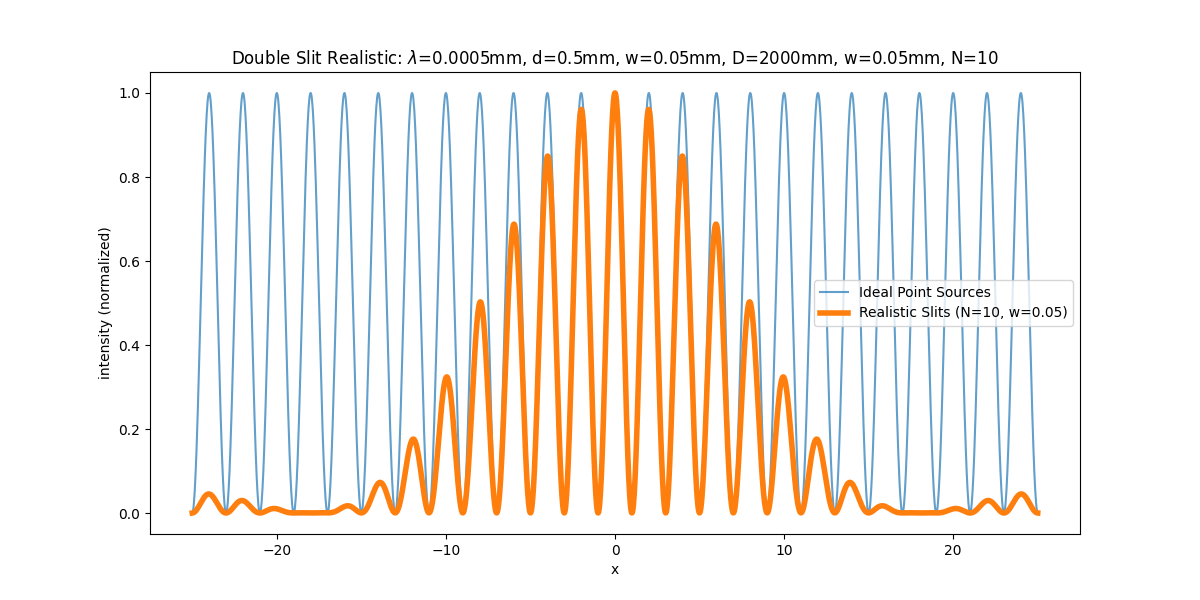
\includegraphics[width=\textwidth]{figures/p4_comparison.png}
        \caption{Realistic slit model}
    \end{subfigure}
    \caption{Comparison between point source double slit ($d=0.5$ mm, $\lambda=0.0005$ mm, $D=2000$ mm).} and realistic doubel slit (with discretization along a continous width $N=10$, $w=0.05$ mm), 
    \label{fig:p4}
\end{figure}

\textbf{Theory:} A realistic double slit model should incorporate both interference and diffraction effects. Theoretical principles suggest that the interference maxima created by the two slits will be modulated by the single-slit diffraction envelope. Consequently, the interference maximas should diminish in intensity further from the central peak, disappearing entirely at the diffraction envelope's null points.

\textbf{Results:} As shown in Figure \ref{fig:p4}, subfigure (a) depicts the ideal double slit modeled with perfect point sources, which produces interference maxima of uniform maximum intensity across the entire screen. Subfigure (b) depicts the realistic slit model, which introduces the finite width $w=0.05$ mm. Comparing the two, the realistic model maintains the exact same interference maximas spacing ($\Delta x$) as the ideal model. However, the intensity of these maximas is now correctly bounded and modulated by the broader single-slit diffraction envelope. This causes the individual fringes to progressively decrease in intensity as they move away from the central maximum, eventually disappearing entirely at the nulls of the diffraction envelope. This behavior demonstrates the physical convolution of interference and diffraction, in full agreement with the realistic theoretical model.

\end{document}
